\documentclass[12pt, dvipsnames, a4paper]{article}
\usepackage{geometry}
\geometry{legalpaper, margin=0.5in}
\usepackage{xcolor}
\usepackage{lipsum,etoolbox}
\usepackage{xspace} 
\usepackage[normalem]{ulem}
\usepackage{vwcol}
\usepackage{cancel}
\usepackage{enumitem}
\usepackage{amsmath}
\usepackage{caption}
\usepackage{graphicx}
\usepackage{amsfonts}
\usepackage{float}
\usepackage{multicol}
\usepackage{hyperref}
\usepackage{listings}
\usepackage{textcomp}
\usepackage{lstautogobble}
\usepackage[parfill]{parskip}
\usepackage{tikz-qtree}
\usepackage{tikz}
\usepackage{hyperref}
\usepackage[english]{babel}
\usepackage[autostyle, english = american]{csquotes}
\MakeOuterQuote{"}
\usetikzlibrary{decorations.pathreplacing}
\usetikzlibrary{decorations.pathreplacing}
\tikzset{every tree node/.style={minimum width=4cm,draw,circle},
         blank/.style={draw=none},
         edge from parent/.style=
         {draw,edge from parent path={(\tikzparentnode) -- (\tikzchildnode)}},
         level distance=1.5cm}

%% Genearl %%
\renewcommand{\thesection}{\arabic{section}}


%% For convenience %%
\newcommand{\code}[1]{\texttt{#1}}
\newcommand{\bcode}[1]{\texttt{\textbf{#1}}}
\newcommand{\balert}[1]{\textbf{\alert{#1}}}
\newcommand{\rarrow}{$\Rightarrow$}
\newcommand{\tab}[1][0.5cm]{\hspace*{#1}}
\newcommand{\deepemphasis}[1]{\underline{\textbf{\Large{#1}}}}
\newcommand{\bfemph}[1]{\textbf{\emph{#1}}}
\newcommand{\OR}[0]{\lvert \: \rvert}

%% Colours %%
\definecolor{mLightBrown}{HTML}{EB811B}
\definecolor{mLightGreen}{HTML}{14B03D}

%% Pseudocode %% 
\lstdefinelanguage{pseudo}
{
	keywords=[1]{
		let,
		class,
		new,
		loop,
		until,
		end,
		if,
		else,
		then,
		return,
		while,
		for,
		to,
		fun,
		break,
		and,
		true,
		false,
		or,
		do,
		max,
		min,
		elif,
	},
	keywordstyle=[1]\color{black}\bf,
	keywords=[2] {
		invariant,
		precond,
		postcond
	},
	keywordstyle=[2]\color{blue}\bf
}

\lstset{
	breaklines		=	true,
	language 		= 	pseudo,
	basicstyle		=	\ttfamily,
	mathescape		=	true,
	escapeinside	=	||,
	tabsize			=	2,
	numbers			=	left,
	commentstyle	=	\color{OliveGreen},
	stringstyle		=	\color{mLightBrown},
	upquote			=	true,
	morestring		=	[b]',
	moredelim		=	[l][\rmfamily\itshape]{@},
	comment			=	[l]{//},
	morecomment		=	[s]{/*}{*/},
	commentstyle=\color{Gray}\ttfamily,
	showstringspaces=	false,
	showtabs		=	false,
	autogobble
}

%% Other %%
\setcounter{secnumdepth}{5}
\setcounter{tocdepth}{5}

% \patchcmd{<cmd>}{<search>}{<replace>}{<success>}{<failure>}
\patchcmd{\abstract}{\titlepage}{\titlepage% Insert ToC-writing after starting a titlepage
  \addcontentsline{toc}{chapter}{Abstract}}{}{}
\setcounter{secnumdepth}{3}
\setcounter{tocdepth}{3}

% Keywords command
\providecommand{\keywords}[1]
{
  \small	
  \textbf{\textit{Keywords---}} #1
}


%**************************************************************************************************************%
%______________________________________________________________________________________________________________%
\begin{document}
\title{\textbf{EECS 4314 - Bit Theory\\Concrete Architecture Report}}
\date{\Large \today}
\author{
	\large \textbf{Amir Mohamad}\\ \small amohamad@my.yorku.ca\\\\
	\large \textbf{Arian Mohamad Hosaini}\\ \small mohama23@my.yorku.ca\\\\
	\large \textbf{Dante Laviolette}\\ \small dantelav@my.yorku.ca\\\\
	\large \textbf{Diego Santosuosso Salerno}\\ \small nicodemo@my.yorku.ca\\\\
	\large \textbf{Isaiah Linares}\\ \small isaiah88@my.yorku.ca\\\\
	\large \textbf{Joel Fagen}\\ \small joefagan@my.yorku.ca\\\\
	\large \textbf{Misato Shimizu}\\ \small misato1@my.yorku.ca\\\\
	\large \textbf{Muhammad Hassan}\\ \small furquanh@my.yorku.ca\\\\
	\large \textbf{Yi Qin}\\ \small aidenqin@my.yorku.ca\\\\
	\large \textbf{Zhilong Lin}\\ \small lzl1114@my.yorku.ca\\\\
	\large York University\\
}
\maketitle
\newpage
\hspace{0pt}
\vfill
\begin{abstract}
	Concrete Architecture identifies the relationships between the subsystem and components inside the project. It includes what the system does, how it will implement the functionality, identification of significant components and connectors and realization of architecture mechanisms. The concrete architecture will investigate the responsibilities, component interaction, control and data flow. Interprocess communication is the methodology that allows the processes to communicate with each other and synchronize their actions. This communication between the processes can also be called a method of cooperation between processes. There are several advantages of using IPC. First, it is convenient because it allows a single user to work on many tasks simultaneously. IPC can divide the extensive system’s functions into small processes or threads. These small processes can also speed up the processes of each execution and simultaneously execute the other processes. These processes will share the data they are using concurrently, reducing the time for processes to reload the data into the memory. In FreeBSD, the IPC model will provide access to communication networks such as the Internet. For 4.2BSD, the interprocess-communication facilities were intended to provide a sufficiently general interface to allow network-based applications to be constructed independently of the underlying communication facilities. To allow multiprocess programs, FreeBSD uses UNIX pipe. These pipes force systems to be designed with a contorted structure. The pipe contains four properties to interact with the data being used in the system. The four properties are:
	\begin{itemize}
		\item In-order delivery of data.
		\item Unduplicated delivery of data.
		\item Unduplicated delivery of data.
		\item Reliable delivery of data and connection-oriented communication.
	\end{itemize}

	In FreeBSD, the system must support communication networks that use different sets of protocols, naming conventions, hardware, and so on. In this case, the IPC contains the communication domain. A communication domain embodies the standard semantics of communication and naming, allowing the system to connect to different networks with different standards. To communicate across networks, FreeBSD uses sockets. Compared to the pipe method, sockets have not only the properties pipes have, but they also have properties such as preserving message boundaries and supporting out-of-band messages.
	\\\\
	\keywords{concrete architecture, conceptual architecture, IPC, FreeBSD, pipes, sockets}
\end{abstract}
\vfill
\hspace{0pt}
\newpage
\tableofcontents
\clearpage

\section{Introduction}
As we have discussed, the operating system is one of the essential parts of all kinds of computers, and it is responsible for managing the whole computer system. Due to this complex mission, the operating system needs the support of several subsystems to help it finish the job perfectly. One of those main subsystems is the interprocess communication system, also known as IPC, which is the target we will discuss.
Interprocess communication can be defined as the mechanism that the operating systems provide to manage the data shared between processes in the operating system.
The principle of interprocess communication is pretty simple.
While the processes or applications are trying to transfer data, the process that requests the data will be considered a client, and the process that sends the data will be the server.
Most of the applications can be both client and server.
There are three goals for the interprocess-communication model. The first was providing access to communication networks such as the Internet.
The second goal was to allow multiprocess programs, such as distributed databases, to be implemented.
The third goal is to provide new communication facilities for constructing local-area network services, such as file servers. These facilities are designed to support: Transparency which ensures that the communication between processes can be on different machines, Efficiency, which provides the applicability of any IPC facility and Compatibility ensures the existing naïve processes should be usable in a distributed environment without change.

\subsection{Overview}
The report will analyze the concrete architecture of the FreeBSD operating system's interprocess communication(IPC) system.  We will deeply explore the derivation process and learn about the architecture of IPC.
After that, the report will analyze the reflection and use case to help understand IPC from another point of view.
Finally, there will be a conclusion summarizing the limitations we met in the exploration and the lesson we have learnt from this process.
\clearpage

\section{Derivation Process}
\begin{figure}[!htb]
	\center
	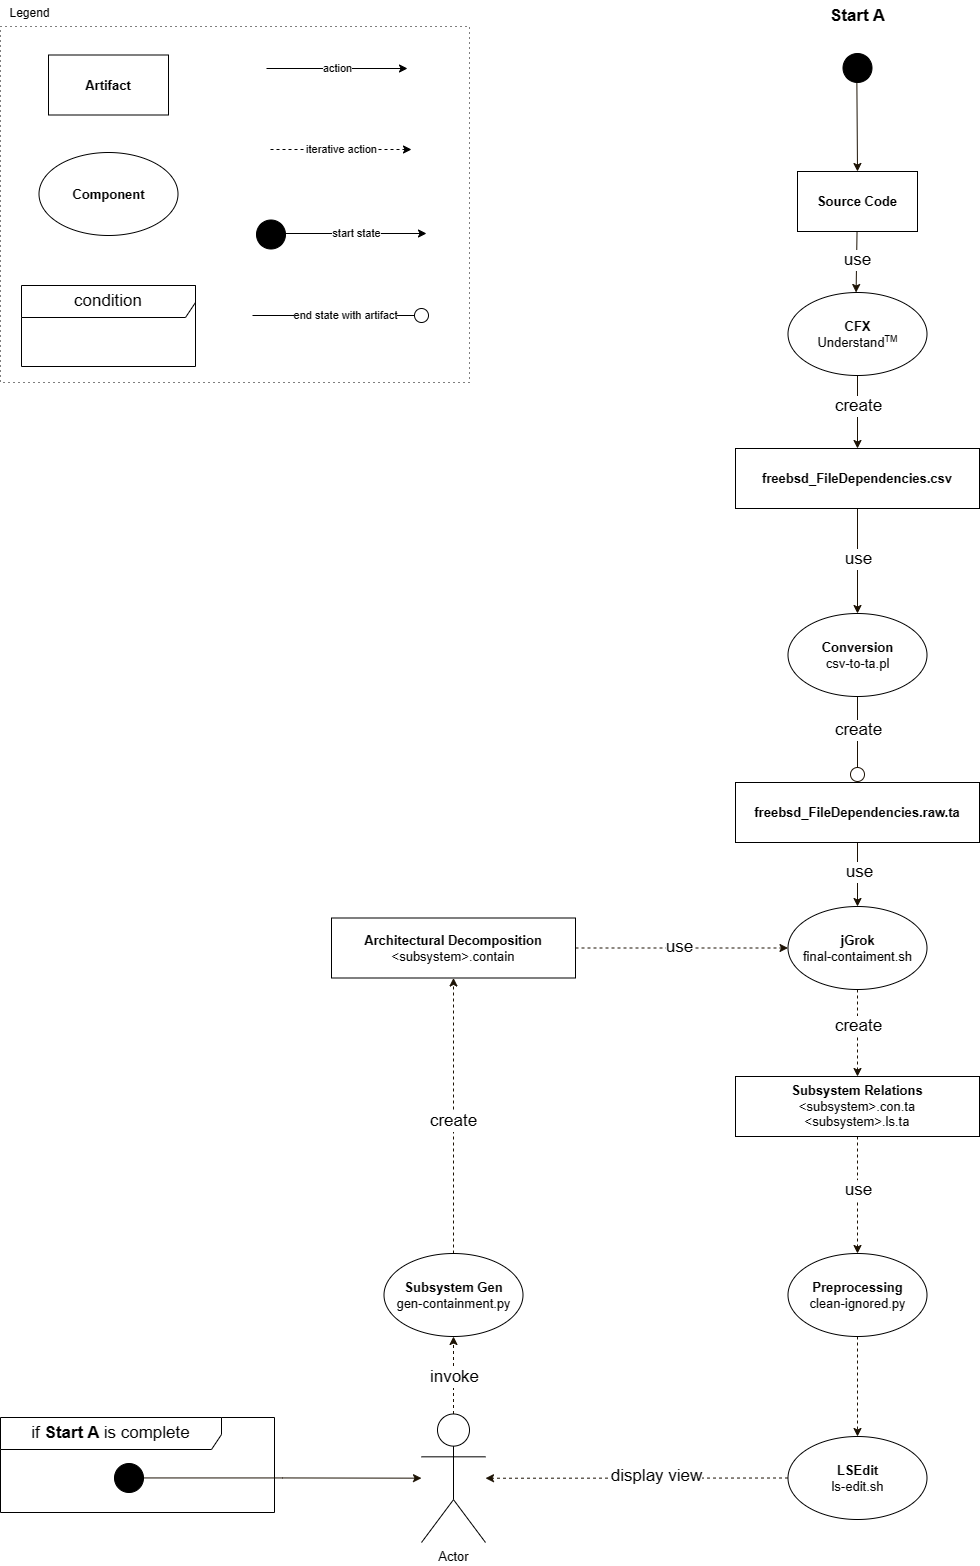
\includegraphics[width = 290pt]{assets/derivation_diagram.png}
	\caption{Concrete architecture derivation process \cite{derivation}}
\end{figure}
Unlike the process of understanding conceptual architecture, which requires mainly documentation reviews, understanding concrete architecture can be more challenging and complicated as it requires source code observations. To have better understanding of FreeBSD’s concrete architecture, we followed extraction steps, and they are shown as a derivation process in a figure above.
After downloading FreeBSD source code, we use a source code extractor (\code{cfx}), Understand, which retrieves relations from the source code (e.g., control and data flow dependencies, relations among function calls). Here, we obtain a file, \code{freebsd\_FileDependencies.csv} which has been produced by Understand. By running a Perl command to convert the csv file into a \code{raw.ta} file using \code{csv-to-ta.pl}, software, called \code{jGrok}, figures out their subsystem relations. After filtering dependencies by running \code{clean-ignored}.py, a graphical landscape editor, \code{LSEdit}, takes a role of visualizations for the extracted relations. Our task here is to manually observe those visualized diagrams using \code{ls-edit.sh}, and decompose subsystems hierarchically and pass the decomposed architectural structure to \code{jGrok}. We repeat these processes until we reach the point where the subsystem structure is understood in clear and detailed manners.
\clearpage
\section{Results}
\subsection{Conceptual Architecture}
Figure 2 below is the conceptual architecture derived in assignment 1. We won't go into much detail but we will have it as reference as we analyze the concrete architecture in comparison.

\begin{figure}[!htb]
	\center
	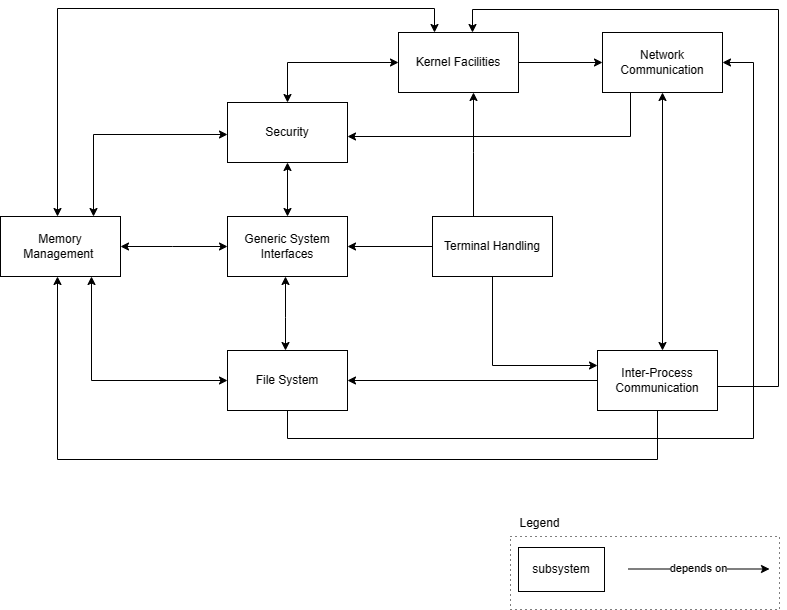
\includegraphics[width = 390pt]{assets/conceptual-architecture.png}
	\caption{Conceptual architecture of FreeBSD subsystems}
\end{figure}
\subsection{Concrete Architecture}

The final iteration of our derivation process resulted in a concrete dependency diagram of the FreeBSD subsystems in Figure 3. Notably, we discovered several new dependencies represented by dashed red lines and unexpected bidirectional dependencies, depicted by hollow arrows. We also discovered a few removed dependencies, represented by crossed arrows. Furthermore, we identified two new subsystems, Crypto and Subroutines. To our surprise, majority of our existing dependencies in our conceptual diagram in Figure 2 stayed consistent, besides the various new divergences. Later in the report, we will analyze a few of these divergences in the IPC subsystem.

\begin{figure}[!htb]
	\center
	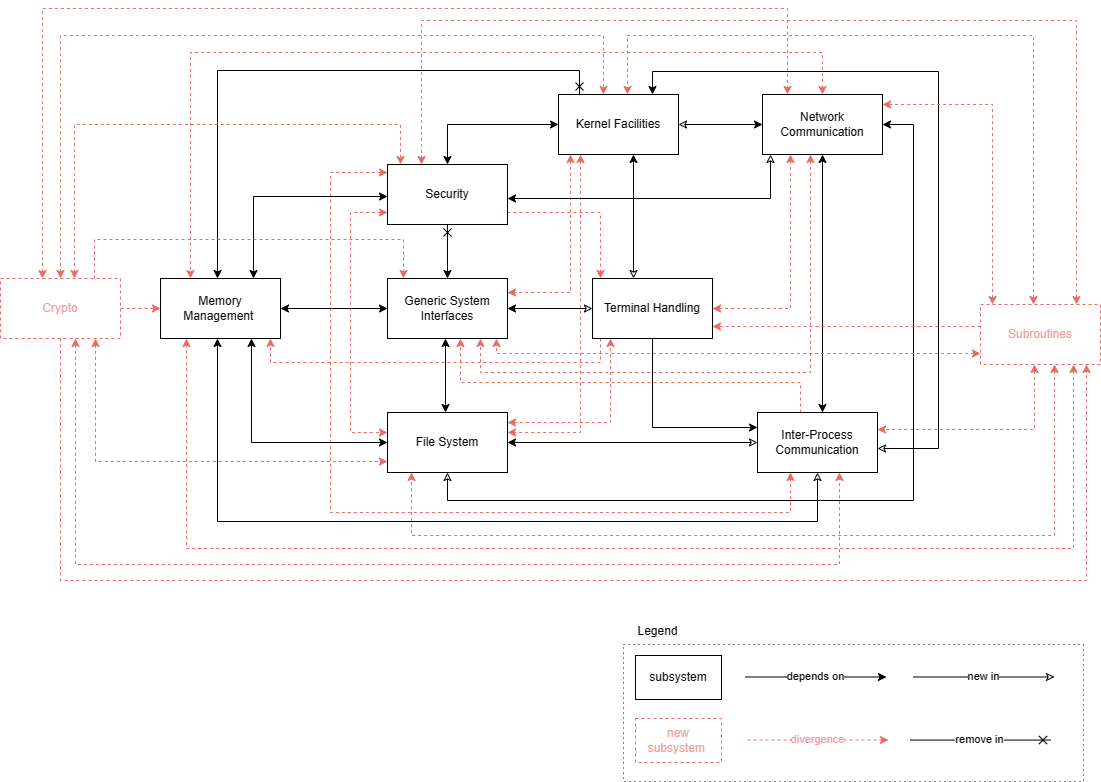
\includegraphics[width = 390pt]{assets/concrete-architecture.png}
	\caption{Concrete architecture of FreeBSD subsystems}
\end{figure}
\clearpage
\subsection{Concrete Inter-Process Communication Architecture}

The derivation process of the IPC subsystem in FreeBSD revealed a few new dependencies and subsystems. We will review some of the subsystems that IPC depends on and their functionality. The Security subsystem supports IPC, performing security audits on IPC mechanisms to ensure the system is traceable and secure \cite{audit}. The Generic System Interfaces subsystem provides the necessary data structures for implementing IPC. For example, IPC uses the message queue data structure defined in \code{sys/msg.h} and the shared memory data structure \code{sys/shm.h} to represent data for various implementations logically. The new Subroutines subsystem offers support functions for complex tasks. For instance, IPC uses system calls indirectly using \code{subr\_syscall.c} when interacting with the kernel. Additionally, IPC depends on Crypto, which indirectly utilizes its cryptography functions to provide secure communication by encrypting and decrypting messages between processes. Understanding these dependencies provides valuable insights into the workings of the complex monolithic architecture of the FreeBSD kernel.

\begin{figure}[!htb]
	\center
	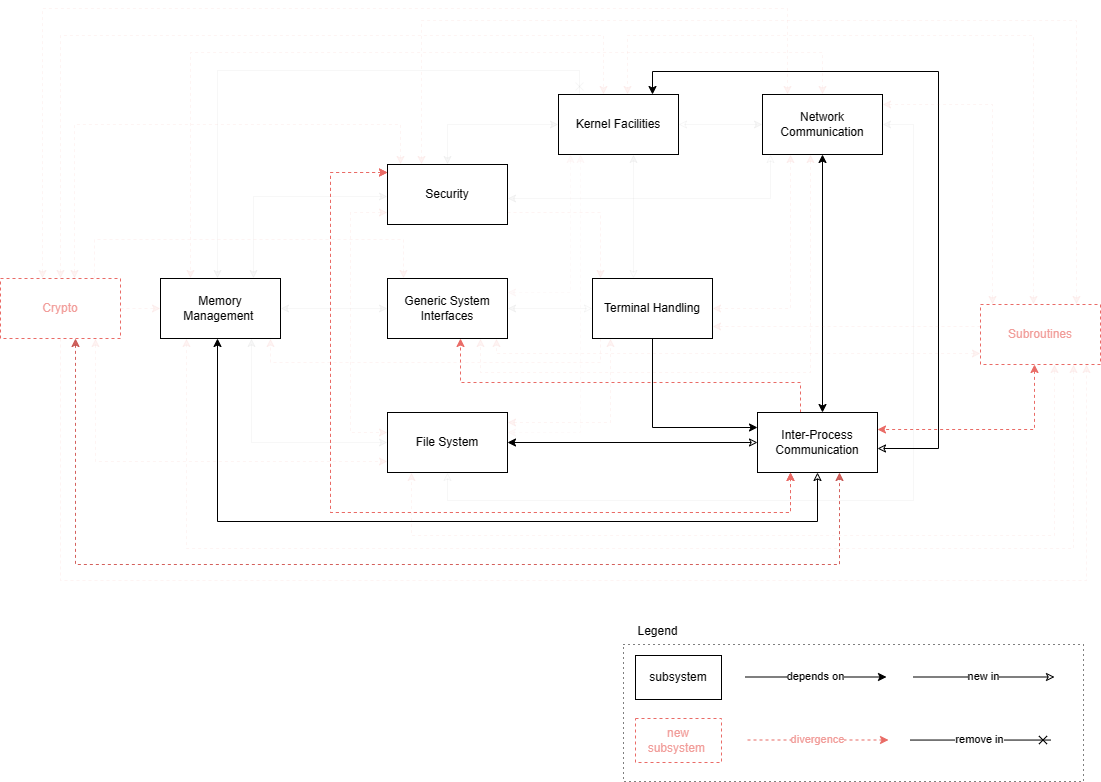
\includegraphics[width = 390pt]{assets/ipc-concrete-architecture.png}
	\caption{Concrete architecture of FreeBSD IPC subsystem}
	\label{fig:concreteIPC}
\end{figure}
\subsection{Top Level Kernel Dependencies}

We created a custom script, \code{count-links.py} as a part of our derivation process to see how the FreeBSD kernel depended on the top level modules. We found that the kernel depended on the top level modules \code{lib}, \code{stand}, and \code{contrib} very strongly. All these dependencies had 1k to 6K+ use cases in the kernel. The kernel depended on the \code{stand} module, where the boot loader sources reside, the most with over 10k links.
\begin{figure}[!htb]
	\center
	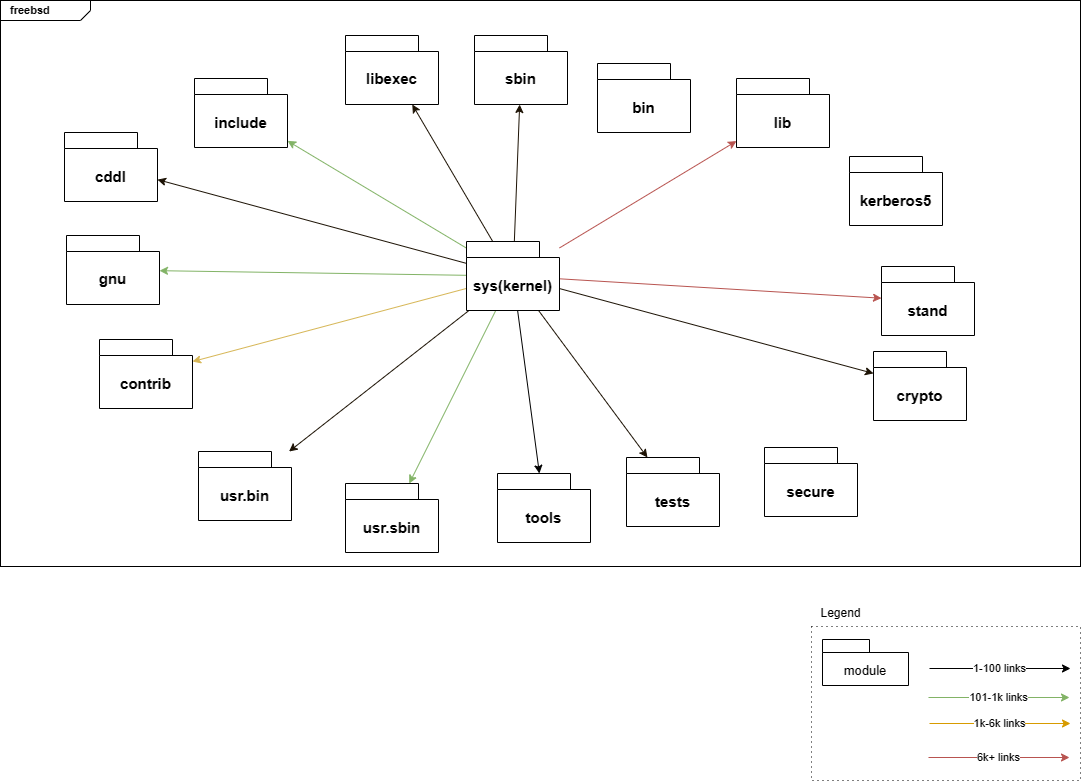
\includegraphics[width = 390pt]{assets/kernel-dependencies.png}
	\caption{Kernel dependencies on top level modules in FreeBSD}
\end{figure}
\clearpage
\section{Architecture}
\begin{figure}[!htb]
	\center
	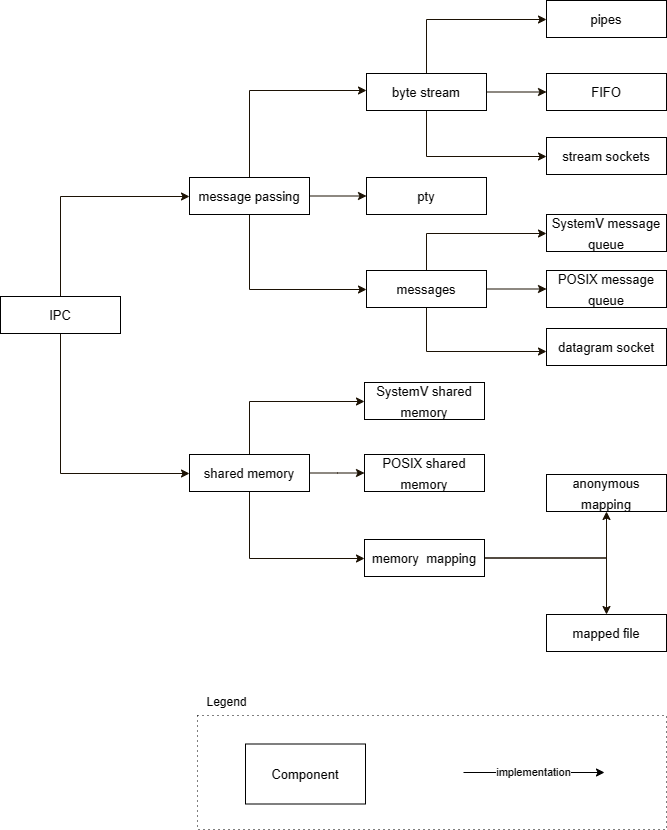
\includegraphics[width = 290pt]{assets/ipc-implementations.png}
	\caption{The IPC implementations breakdown of FreeBSD}
\end{figure}
\subsection{Networking Inter-Process Communication}
The network IPC facilities are layed on top of the networking facilities, and this heavy coupling is shown in the conceptual architecture and confirmed in the concrete architecture we derived. Data from the application is sent through the socket layer to the networking layer, and data coming in flows from the networking layer through the socket, and then into the receiving application.  State required by the socket layer is fully encapsulated within it, whereas any protocol-related state is maintained in data structures that are specific to the supporting protocols. The system-call interface routines manage the actions related to a system call, collecting parameters, and converting user data into the format expected by the socket layer routine. Socket layer routines directly manipulate socket data structures and manage the synchronization between asynchronous activities.
\begin{figure}[!htb]
	\centering
	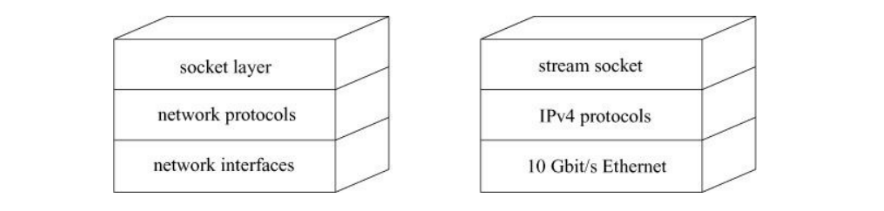
\includegraphics[width=500pt]{assets/IPC_Net_ARCH.png}
	\caption{Networking IPC Layered Architecture}\cite{mckusick}
\end{figure}
\subsection{Local Inter-Process Communication}
As well as network sockets, local interprocess communication is provided inside the kernel, in the form of semaphores, shared memory, and message queues. Initially, these mechanisms were provided by \code{System V}, and they are often referred to as \code{System V} semaphores, mutexes, and shared memory. There are some applications that use the \code{System V} implementation, such as \code{PostgreSQL} or \code{X11}. Later, \code{POSIX} was added to the kernel, and improves upon System V by introducing file descriptors. \code{POSIX}’s implementations of semaphores and shared-memory objects have replaced \code{System V}’s implementations in many applications. For example, Capsicum uses its own version of the \code{POSIX} shared-memory interface which links a file descriptor with an anonymous \code{vm\_object} and allows multiple processes to share this object through the file descriptor.

Previously, UNIX used the filesystem namespace to allow processes to rendezvous with each other and share their resources. But FreeBSD used the \code{System V} IPC, which introduced a new key-based namespace. Using \code{ftok()}, it would generate a key for a process based on its pathname. Multiple processes with the same pathname would get the same key. Using that key, a process would then create or get a specific object using the get call, using the \code{IPC\_CREAT} flag to specify whether the object is being created or retrieved. The table below shows the \code{POSIX} and \code{System V} APIs for how they handle IPC objects.

\begin{figure}[!htb]
	\centering
	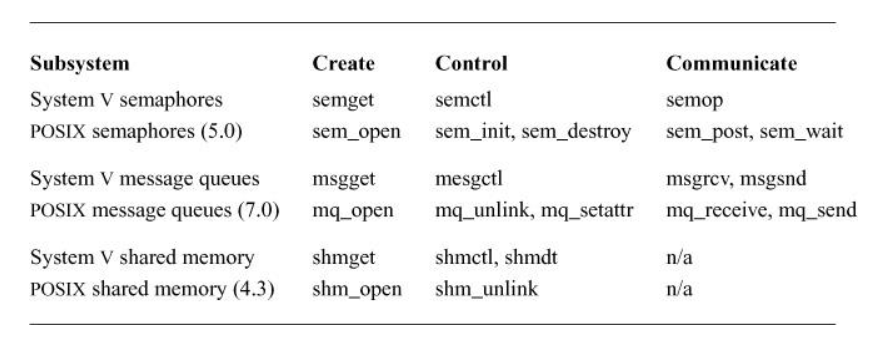
\includegraphics[width=290pt]{assets/localipc1.png}
	\caption{Comparison of APIs between \code{System V} and \code{POSIX}} \cite{mckusick}
\end{figure}

Pipes come from the \code{POSIX} standard, and are a common way to set up an interprocess communication channel for one process to send data to another in a byte-stream. Pipes are unidirectional, meaning they can only send data from one process to another and not in reverse. Contrast this with sockets (also in the \code{POSIX} standard), where data flow is bidirectional. A group of processes, aka a job, are connected by the shell via pipes. The output of the first process is fed into the second process, then the output of the second process is fed into the third, and so on. This is often referred to as a pipeline, and is reminiscent of the pipe and filter architecture style.

\begin{figure}[!htb]
	\centering
	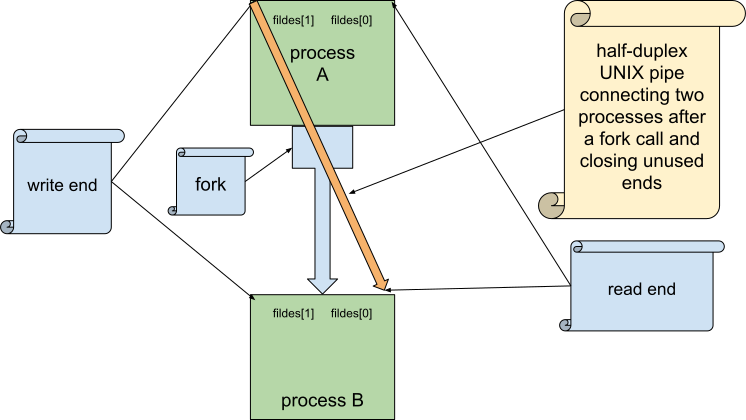
\includegraphics[width=290pt]{assets/localipc2.png}
	\caption{A diagram of the pipeline architecture in \code{POSIX}} \cite{rytarowski}
\end{figure}

In \code{POSIX}, \code{pipe()} takes an array of two integers. \code{fildes[1]} is used for writing, and \code{fildes[0]} is used for reading. In the above diagram, process B is forked from process A, and the written data from process A is fed through the pipe into process B. If it returns successfully, it writes file descriptors on each end of the pipeline. Otherwise, it returns \code{-1}.

\clearpage
\section{Reflextion Analysis}
Now to start our reflection analysis of the introduced divergences from the conceptual architecture  we will look at the dependencies from Inter-Process Communication to General System Interfaces. The General System Interfaces subsystem has a large amount of facilities and data structures used by IPC so we will only go over a couple. First, we will look at the dependency between \code{uipc\_socket.c} and \code{jail.h}. The \code{uipc\_socket.c} file implements a very large amount of socket facilities and is an extremely large file with many dependencies. The \code{jail.h} file implements the jail and prison data structures. This dependency was introduced because previously, interaction with IPv6 was not well-defined, and might be inappropriate for some environments. So what the author, rwatson, did to solve this was modify jail to limit creation of sockets to: UNIX domain sockets, TCP/IP (v4) sockets, and routing sockets. At the time of this change, this functionality was enabled by default, and toggleable using a variable in \code{jail.h}.
\begin{figure}[!htb]
	\centering
	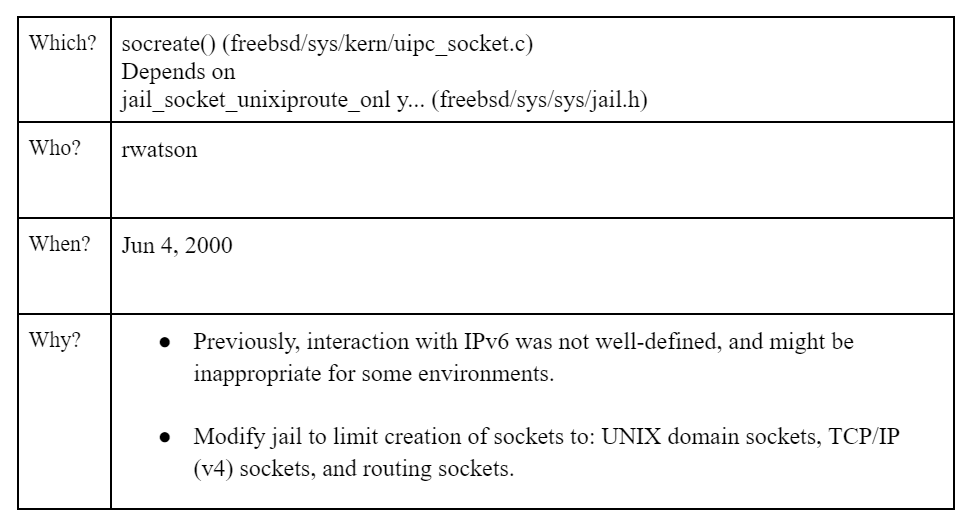
\includegraphics[width=290pt]{assets/IPC_Jail.png}
	\caption{InterProcessCommunication $\longrightarrow$ GeneralSystemInterfaces \code{jail.h} Reflection Analysis}
\end{figure}

This next dependency is between \code{uipc\_socket.c} and \code{sx.h}; which implements the lock data structure / facilities. To give some context, the sx in \code{sx.h} stands for shared/exclusive and shared/exclusive locks are used to protect data that are read more often than they are written. The key difference between shared/exclusive locks and regular read-write locks is that they do not implement priority propagation like mutexes and reader/writer locks to prevent priority inversions. This change was also done by rwatson and was well documented. This change was an optimization which resulted in: Marginally better performance, Better handling of contention during simultaneous socket I/O across multiple threads, and A cleaner separation between the different layers of locking in socket buffers.

\begin{figure}[!htb]
	\centering
	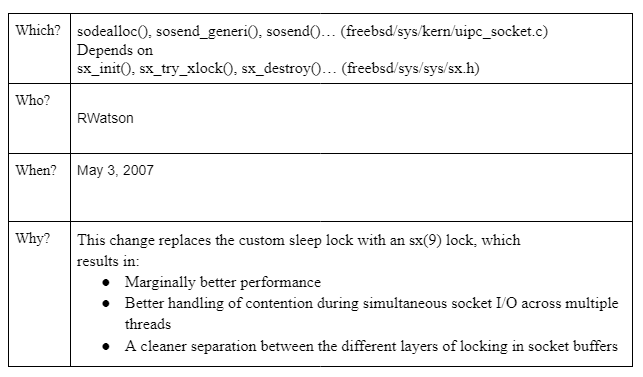
\includegraphics[width=290pt]{assets/IPC_Sx.png}
	\caption{InterProcessCommunication $\longrightarrow$ GeneralSystemInterfaces \code{sx.h} Reflection Analysis}\cite{sx}
\end{figure}

\subsection{IPC dependence on the Security Subsystem}
Another dependency that we discovered in the process of extracting the concrete architecture is that IPC depended on the Security subsystem. The Security subsystem in FreeBSD is responsible for enforcing security policies and mechanisms at various level of the system, including network security, user authentication, access control, and system integrity.

The IPC subsystem depends on the Security subsystem in two main ways:

\subsubsection{Access Control}
The IPC subsystem relies on the Security subsystem to enforce access control policies for IPC resources such as message queues, shared memory segments, and semaphores. The security subsystem provides mechanism such as file permissions and mandatory access control (MAC) frameworks to restrict access to IPC resources based on user identities, level of privilege the user has and security policies. We did a study of the source code FreeBSD and found the file level dependency that explains this relation of two subsystem:

\begin{figure}[!htb]
	\centering
	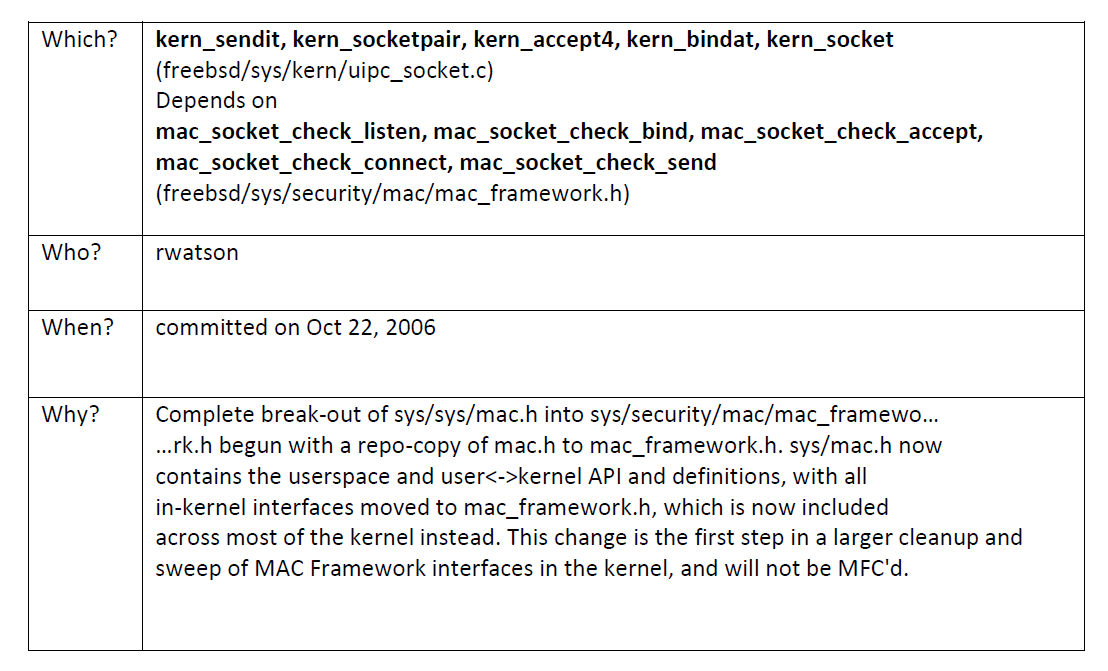
\includegraphics[width=290pt]{assets/4Ws_2.png}
	\caption{InterProcessCommunication $\longrightarrow$ Security \code{mac\_framework.h} Reflection Analysis}
\end{figure}

Here we see that a file named \code{uipc\_socket.c} depends on a header file \code{mac\_framework.h}, that is part of the security subsystem. \code{uipc\_socket.c} contains implementation of socket related functions. This file is responsible for creating, managing, and interacting with sockets for network communication. the reason for the dependency to \code{mac\_framework.h} is that it provides a mechanism for implementing and enforcing mandatory access control policies. Therefore, the inclusion of \code{mac\_framework.h} is essential for ensuring the security of network communication in FreeBSD.

\subsubsection{System Integrity}
It is also essential that the integrity of IPC resources are maintained and that there is no unauthorized modification or tampering. The security subsystem provides mechanisms such for logging and monitoring system activity for this purpose. The auditing subsystem can track various types of system events, including process creation, IPC activity, and file access. We went ahead a tried to find this dependency in the source code and came across the following relation:

\begin{figure}[!htb]
	\centering
	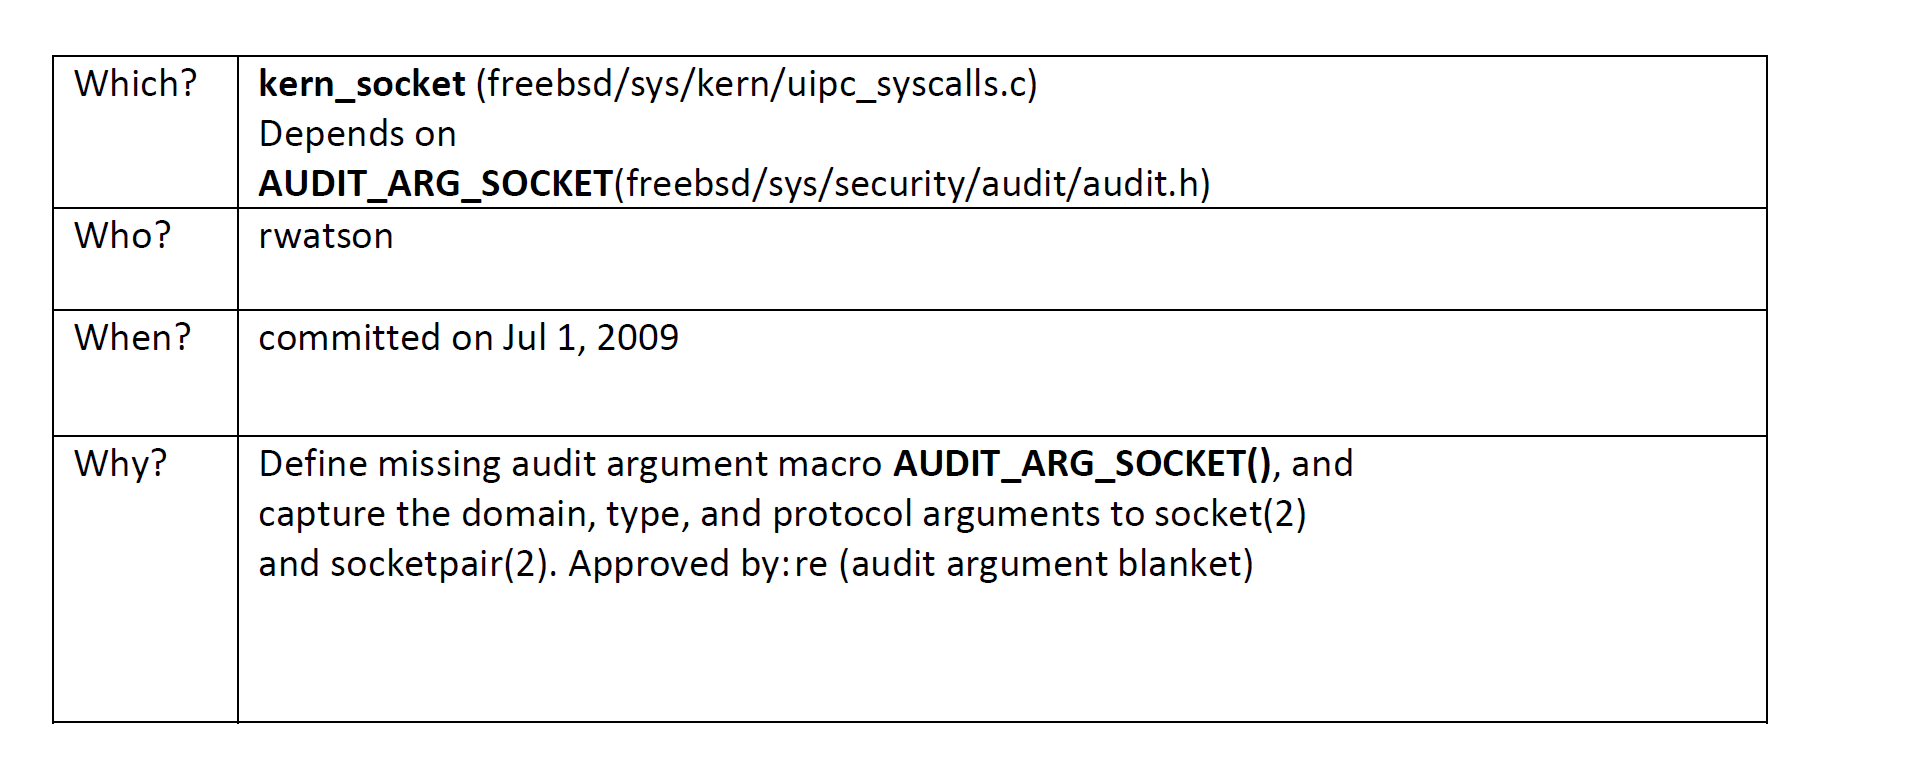
\includegraphics[width=290pt]{assets/4W's_1.png}
	\caption{InterProcessCommunication $\longrightarrow$ Security \code{audit.h} Reflection Analysis}
\end{figure}

The \code{audit.h} header file provides interface for the system's auditing subsystem, which is responsible for logging and monitoring system activity for security and compliance purposes. A file named \code{uipc\_syscalls.c} that is part of the IPC subsystem depends on \code{audit.h} because it contains an important macro called \code{AUDIT\_ARG\_SOCKET()} \cite{audit}. This macro is used to capture the domain, type, and protocol arguments of \code{socket()} and \code{socketpair()} system calls. These arguments are important pieces of information for auditing network activity, as they indicate the type of socket that is being created. This way the OS gains the ability to log socket-related events to system audit trail \cite{audit}. This allows the system administrator to monitor network activity and detect and suspicious behavior \cite{audit}.
\clearpage

\section{Use Cases}
\subsection{Piping In Shell}
The following sequence diagram shows how system calls can be used to pipe the
output of one application to the input of another in FreeBSD, using a shell
as an example program.
\begin{figure}[!htb]
	\advance\leftskip-0.5cm
	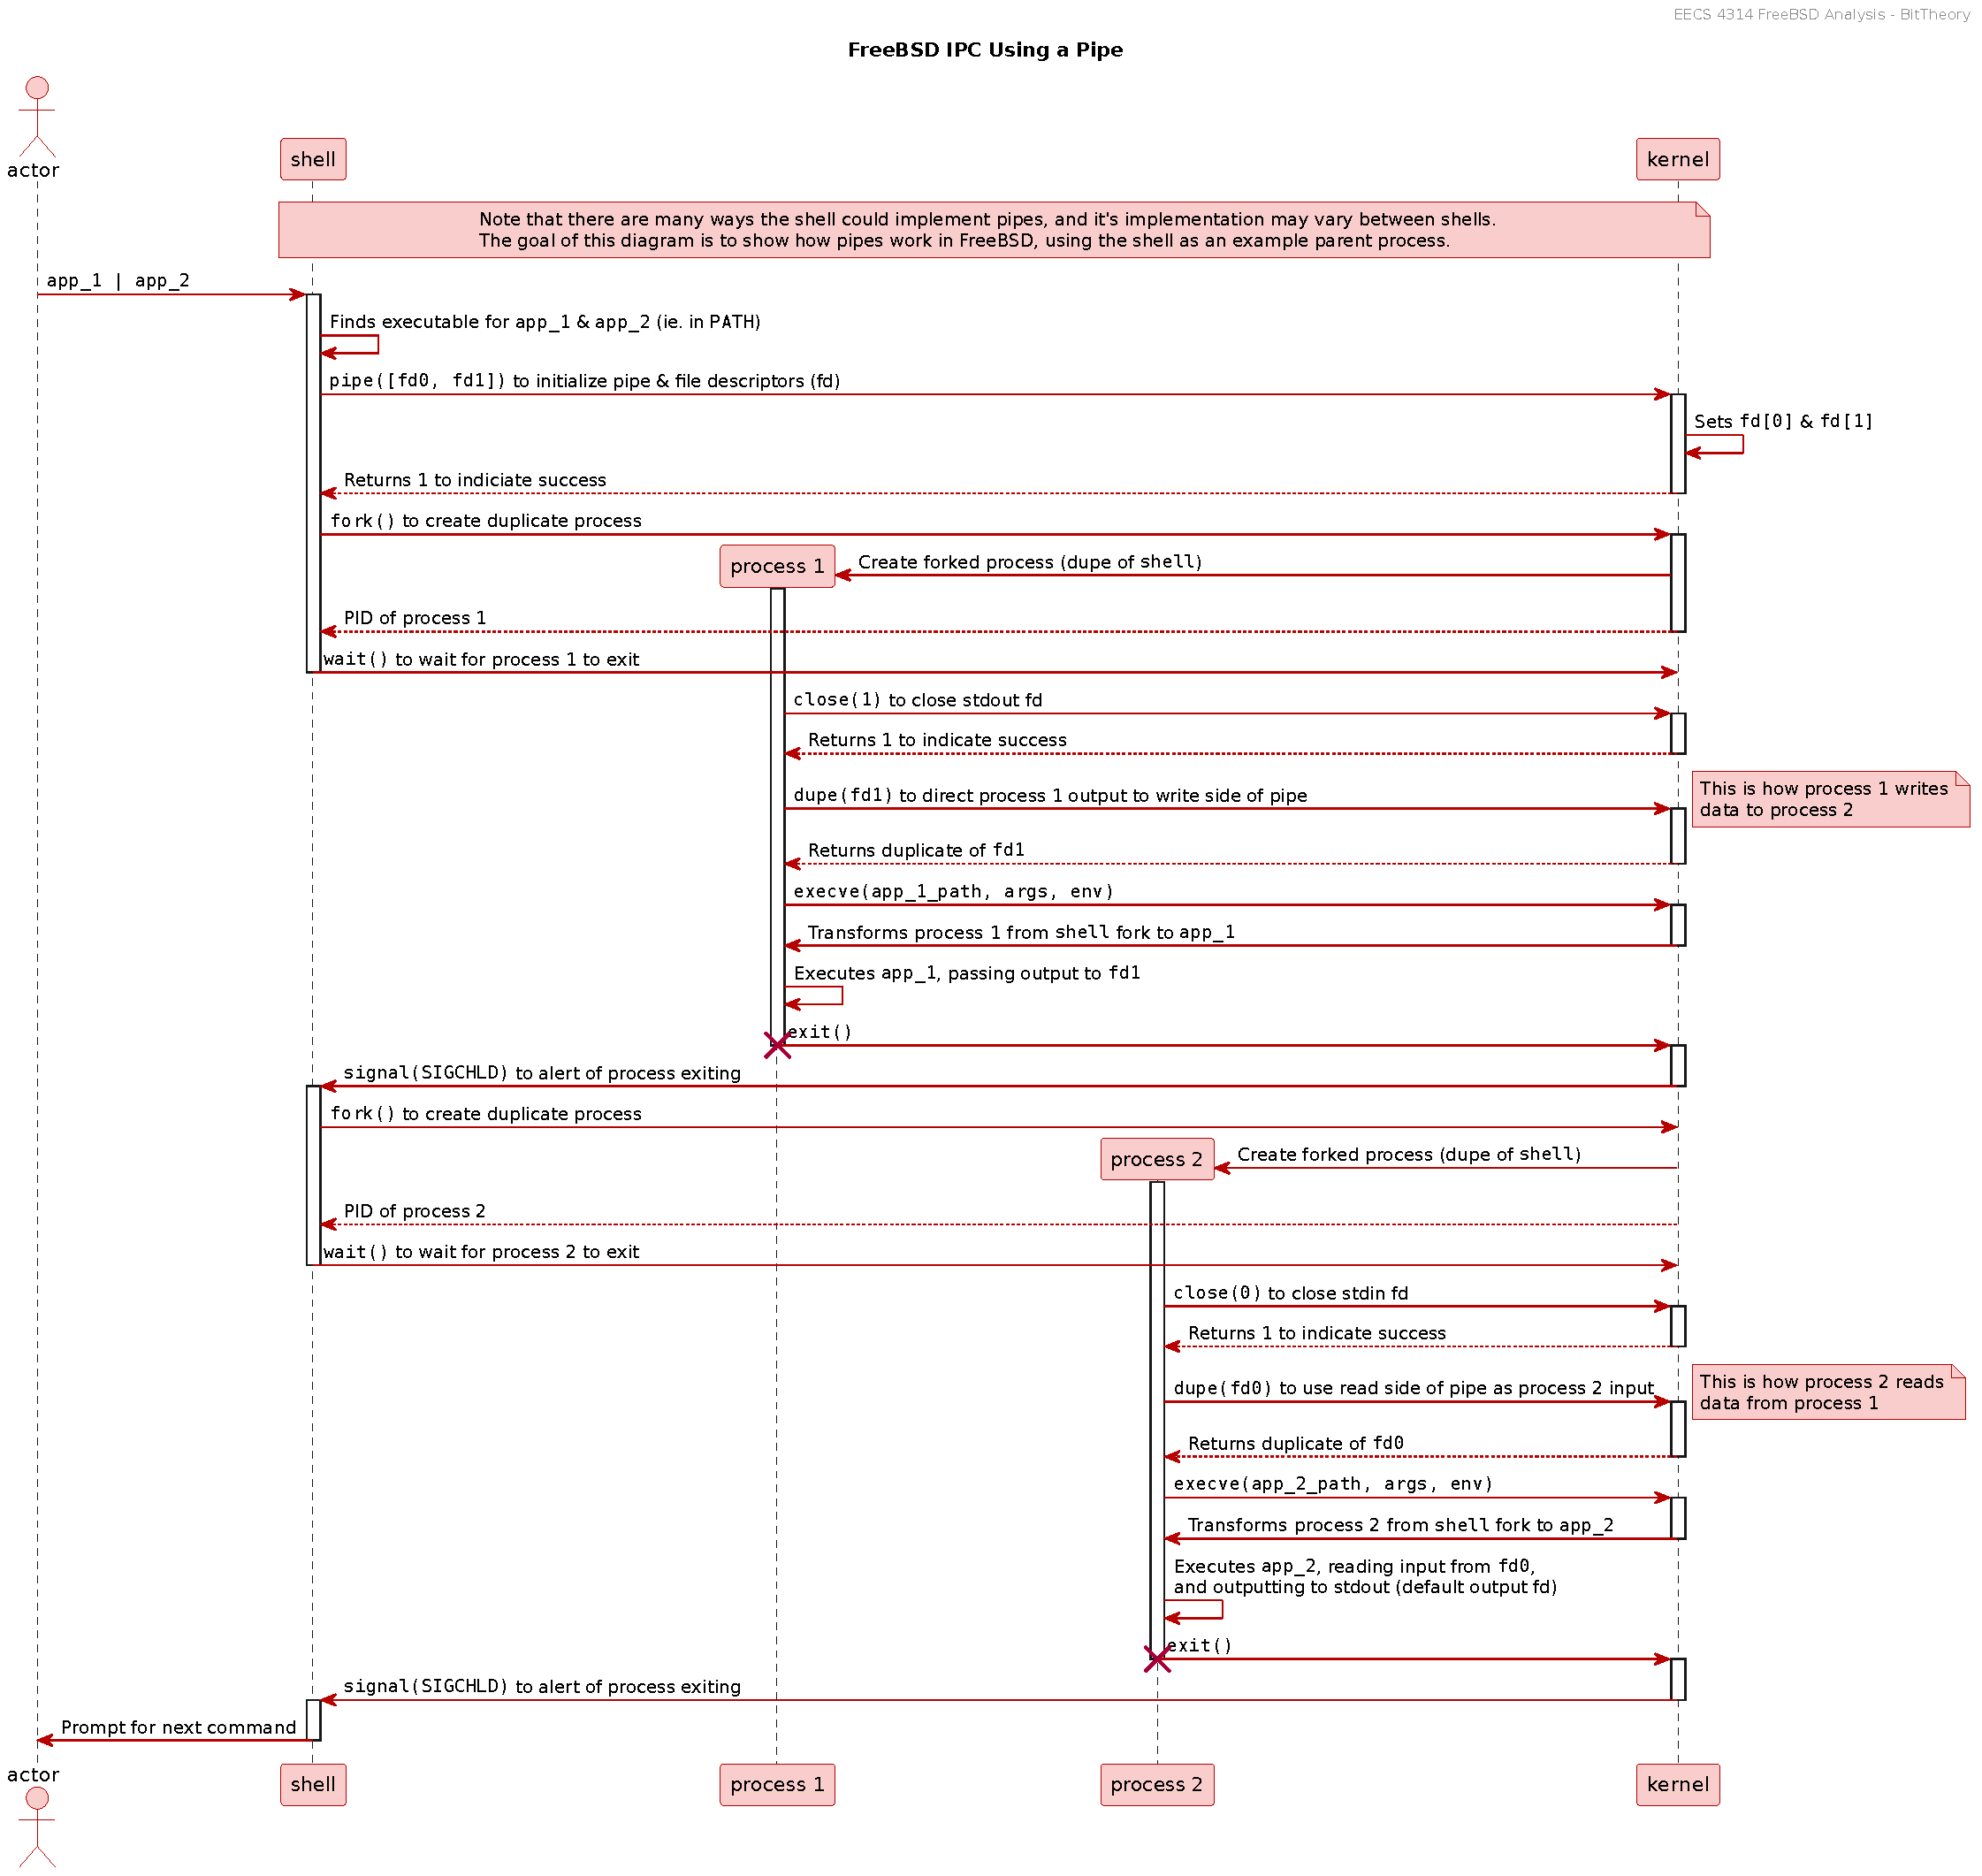
\includegraphics[width = 570pt]{assets/use_case_diagrams/pipe.pdf}
	\caption{Sequence diagram showing pipes being used in the shell for IPC. \cite{pipe}\cite{fork}\cite{wait}\cite{close}\cite{dup}\cite{execve}\cite{signal}\cite{pipe-explained}}
\end{figure}

\clearpage
\section{Conclusion}
In conclusion, the FreeBSD operating system has a powerful and flexible inter-process communication system which allows processes to communicate with each other, both through networks (Networking / Socket IPC) and within local computing environments (Single system / Local IPC).

On one hand, the Socket or networking IPC is a mechanism for communication between processes running on the same system or on different systems connected over a network. In this sense, data from the applications flows through a socket and through a networking layer. The received data, which also comes from the networking layer through the socket, then goes into the application. With sockets, not only do processes not have to run on the same machine in order to communicate between them, they do not even have to run under the same operating system.

Three main types of sockets are supported by the FreeBSD operating system: (1) stream sockets, which provide a connection-oriented, sequential, reliable and bi-directional communication channel; (2) datagram sockets, which provide a message-oriented communication channel in a connectionless manner; and (3) raw sockets, which allow direct access to the low level protocols of the network layer and facilitate sending/receiving network packets.

On the other hand, the single system or local IPC includes an integrated environment of semaphores, message queues, pipes and shared memory regions. Semaphores serve as a synchronization mechanism to allow different processes to access shared memory. Message queues, however, facilitate sending and receiving messages locally in a structured way. Along with pipes, they serve as a buffer that stores messages in a First-In-First-Out (FIFO) manner. These various mechanisms provide low-level access to regions of shared memory and sending/receiving messages between multiple processes.

Overall, FreeBSD provides a variety of IPC mechanisms that allow processes to communicate and coordinate with each other efficiently, whether on the same system or across a network.

\section{Lessons Learned}
After studying the concrete architecture of the IPC (Inter-Process Communication) system of FreeBSD, some of the lessons learned include:

- \textbf{Lesson 1:} The interprocess communication system of FreeBSD is designed to be modular, flexible and scalable, which means that different communication mechanisms between processes can be implemented. This provides a powerful IPC system  for both local and networking environments.

- \textbf{Lesson 2:} As it includes mechanisms such as message queues or stream sockets, the FreeBSD’s IPC system is designed to be reliable and to ensure structured bi-directional communication amongst various local or remote processes.

- \textbf{Lesson 3:} Sockets allow processes to communicate through a network, even within computers with different operating systems. They provide the means for application data to flow through the networking layer, be received by a different process on a different machine, and flow into the application of the new receiving environment.

- \textbf{Lesson 4:} Pipes are used in the shell for interprocess communication in a First-In-First-Out manner. It is a mechanism that allows process communication by sharing an unidirectional stream of data.

- \textbf{Lesson 5:} Overall, the power of the FreeBSD IPC subsystem provides structured, secure and reliable mechanisms for interprocess communication, making it a popular option being widely used in the industry.
\clearpage

\section{Data Dictionary}
\begin{itemize}
	\item{Understand: A source code extractor, used for extracting function relations}
	\item {jGrok: A tool, used for finding subsystem level dependencies}
\end{itemize}

\section{Naming Conventions}
\begin{itemize}
	\item {IPC: Inter-Process Communication}
	      \item{LSEdit: The Landscape Editor}
	\item {CFX: Source Code Extractor}
	\item {FIFO: First in First Out}
	      \item{SX: Shared/Exclusive}
	      \item{I/O: Input/Output}
\end{itemize}

\begin{thebibliography}{00}
	% Using MLA9. If there are too many references, feel free to drop my manpage references %
	\bibitem{bell} Bell-Thomas, A. H. “Interprocess Communication in Freebsd 11: Performance Analysis.” DeepAI, University of Cambridge, 5 Aug. 2020, \href{https://deepai.org/publication/interprocess-communication-in-freebsd-11-performance-analysis}{https://deepai.org/publication/interprocess-communication-in-freebsd-11-performance-analysis}.
	\bibitem{derivation} “BitTheory source code.” README.md, \href{https://github.com/BitTheoryProject/eecs4314-reports/tree/main/a2/src}{https://github.com/BitTheoryProject/eecs4314-reports/tree/main/a2/src}.
	\bibitem{audit} "Chapter 18. Security Event Auditing." FreeBSD Documentation Portal, \href{https://docs.freebsd.org/en/books/handbook/audit/}{https://docs.freebsd.org/en/books/handbook/audit/}.
	\bibitem{close} “FreeBSD Manual Pages.” Close(2), \href{https://man.freebsd.org/cgi/man.cgi?query=close\&sektion=2}{https://man.freebsd.org/cgi/man.cgi?query=close\&sektion=2}.
	\bibitem{dup} “FreeBSD Manual Pages.” Dup(2), \href{https://man.freebsd.org/cgi/man.cgi?query=dup\&sektion=2\&n=1}{https://man.freebsd.org/cgi/man.cgi?query=dup\&sektion=2\&n=1}.
	\bibitem{execve} “FreeBSD Manual Pages.” Execve(2), \href{https://man.freebsd.org/cgi/man.cgi?query=execve\&sektion=2\&n=1}{https://man.freebsd.org/cgi/man.cgi?query=execve\&sektion=2\&n=1}.
	\bibitem{fork} “FreeBSD Manual Pages.” Fork(2), \href{https://man.freebsd.org/cgi/man.cgi?fork(2)}{https://man.freebsd.org/cgi/man.cgi?fork(2)}.
	\bibitem{pipe} “FreeBSD Manual Pages.” Pipe(2), \href{https://man.freebsd.org/cgi/man.cgi?pipe\%282\%29}{https://man.freebsd.org/cgi/man.cgi?pipe\%282\%29}.
	\bibitem{signal} “FreeBSD Manual Pages.” Signal(3), \href{https://man.freebsd.org/cgi/man.cgi?sektion=3\&query=signal}{https://man.freebsd.org/cgi/man.cgi?sektion=3\&query=signal}.
	\bibitem{sx} “FreeBSD Manual Pages.” SX(9), \href{https://man.freebsd.org/cgi/man.cgi?sx(9)}{https://man.freebsd.org/cgi/man.cgi?sx(9)}.
	\bibitem{wait} “FreeBSD Manual Pages.” Wait(2), \href{https://man.freebsd.org/cgi/man.cgi?wait(2)}{https://man.freebsd.org/cgi/man.cgi?wait(2)}.
	\bibitem{mckusick} McKusick, Marshall Kirk. Design and Implementation of the Freebsd Operating System. 2nd ed., Addison-Wesley Professional, 2015.
	\bibitem{pipe-explained} Menon-Sen, Abhijit. “How Are Unix Pipes Implemented?” Toroid.org, 27 Mar. 2020, \href{https://toroid.org/unix-pipe-implementation}{https://toroid.org/unix-pipe-implementation}.
	\bibitem{rytarowski}Rytarowski, Kamil. “Mastering Unix Pipes, Part 1.” Moritz Systems, 26 Nov. 2020, \href{https://www.moritz.systems/blog/mastering-unix-pipes-part-1/}{https://www.moritz.systems/blog/mastering-unix-pipes-part-1/}.
\end{thebibliography}
\end{document}
